% !TeX TS-program = xelatex -synctex=1 -interaction=nonstopmode -shell-escape -output-directory=build %.tex
\documentclass[aspectratio=169]{beamer}

% All my packages are specified and set up in include/format:
\usepackage{include/format}

\title{IoT Crashcourse for Beginners}
\subtitle{Med ESP32}

\author{Jacob Bechmann Pedersen}
\institute{Bechmann Engineering ApS}
\date{\today}

%% Reference settings:
\renewcommand{\figurename}{Figure}
\renewcommand{\tablename}{Table}
\renewcommand{\refname}{References}
\renewcommand{\contentsname}{Contents}
\renewcommand{\listfigurename}{Figures}
\renewcommand{\listtablename}{Tables}
\renewcommand{\lstlistlistingname}{Listings}

\begin{document}

\begin{frame}
	\titlepage
\end{frame}

\begin{frame}{Contents}
	\begin{columns}
	\begin{column}{0.6\textwidth}
		\begin{fitBox}
			\tableofcontents{}
		\end{fitBox}
	\end{column}
	\begin{column}{0.4\textwidth}
		\centering
		\begin{figure}
  			\includesvg[height=0.6\textheight]{assets/svg/ESP32-DevkitC-v4.svg}
  			\caption{ESP32 DevkitC v4, the board we're working with}
  			\label{fig:esp32}
		\end{figure}
	\end{column}
	\end{columns}	
\end{frame}

\section{Who am I?}
\begin{frame}[fragile]{Who am I?}
\begin{columns}
	\begin{column}{0.4\textwidth}
		\begin{center}
		\roundedGfx{0.8\textwidth}{assets/pictures/portrait.png}
		\vspace{0.05\textwidth}
		\begin{columns}
			\begin{column}{0.33\textwidth}
	  			\roundedGfx{\textwidth}{assets/pictures/shiny-hunter.jpg}
			\end{column}
			\begin{column}{0.33\textwidth}
	  			\roundedGfx{\textwidth}{assets/pictures/hackrf.jpg}
			\end{column}
			\begin{column}{0.33\textwidth}
  				\roundedGfx{\textwidth}{assets/pictures/wifi-picture.jpg}
			\end{column}
		\end{columns}
		\end{center}
	\end{column}	

	\begin{column}{0.6\textwidth}
	\begin{textBox}
		Jacob Bechmann Pedersen
			\begin{itemize}
				\item Speaker/Facilitator on Embedded Electronics programming and Arduino workshops
				\item Embedded electronics engineer at DTU Electro, Automation and Control
					\begin{itemize}
						\item Robots, embedded Linux, autonomous systems
					\end{itemize}
				\item Embedded software developer at Oticon
					\begin{itemize}
						\item Applications for hearing aid OS, unit- and device testing
					\end{itemize}
				\item Teacher at MakerCamp
					\begin{itemize}
						\item "Inventors" team - 12-16 y/o
					\end{itemize}
				\item Volunteer in Coding Pirates 2016-2018
				\item Electronic Design Engineer (AU, 2019)
				\item Started with Arduino in 2014
			\end{itemize}
	\end{textBox}
	\end{column}
\end{columns}	
\end{frame}

\section{Purpose}
\begin{frame}{Purpose}
	\begin{textBox}
		\begin{itemize}
			\item To understand the basic principles of IoT
			\begin{itemize}
				\item Topologies
				\item Protocols i. e.:
				\begin{itemize}
					\item HTTP
					\item Websockets
					\item MQTT
				\end{itemize}
			\end{itemize}
			\item To program simple implementations
			\begin{itemize}
				\item On ESP32
				\item With the Arduino platform
				\item In VSCode
			\end{itemize}
		\end{itemize}
	\end{textBox}
\end{frame}

\section{Resources}
\begin{frame}{Resources}
	\begin{textBox}
	Useful links:
		\begin{itemize}
			\item \url{https://github.com/iakop/IoT-Crashcourse}
			\begin{itemize}
				\item Presentation and code for this workshop
			\end{itemize}
			\item \url{https://code.visualstudio.com/}
			\begin{itemize}
				\item Download for Visual Studio Code
			\end{itemize}
			\item \url{https://platformio.org/}
			\begin{itemize}
				\item Download for PlatformIO
			\end{itemize}
			\item \url{https://www.arduino.cc/en/reference}
			\begin{itemize}
				\item Reference on keywords in Arduino
			\end{itemize}
			\item \url{http://mqtt-explorer.com/}
			\begin{itemize}
				\item MQTT client to explore topics on a broker
			\end{itemize}
			\item \url{https://nodered.org/}
			\begin{itemize}
				\item Editor based tool for flowbased IoT programming
			\end{itemize}
		\end{itemize}
	\end{textBox}
\end{frame}

\section{Setup of VSCode and PlatformIO}
\begin{frame}
	\sectiontitle{assets/pictures/vscode-logo.png}{\insertsectionhead}
\end{frame}

\subsection{Setup VSCode}
\begin{frame}{Setup VSCode}
\begin{columns}
	\begin{column}{0.5\textwidth}
		\begin{figure}
  			\roundedGfx{\textwidth}{assets/pictures/vscode-dl.png}
  			\caption{The \tthigh{Visual Studio Code} download page has versions for many different architectures, typically the default button will download the right installer}
  			\label{fig:vscode-dl}
		\end{figure}
	\end{column}
	\begin{column}{0.5\textwidth}
		\begin{textBox}
			\begin{itemize}
				\item Download Visual Studio Code from the link:
				\begin{itemize}
					 \item \small\url{https://code.visualstudio.com/Download}
				\end{itemize}
				\item \tthigh{Click the big button for you OS}
				\item Run the installer, this should go without a hitch
				\item \ttwarn{IF} that doesn't work, you can try:
				\begin{itemize}
					\item Windows:
					\begin{itemize}
						\item If you don't have admin rights, you can download the \tthigh{User Installer} (typically x64-version)
					\end{itemize}
					\item Linux:
					\begin{itemize}
						\item If you don't use Ubuntu try checking your package managers repositories, or try the \tthigh{CLI} installer
					\end{itemize}
					\item Mac OS X:
					\begin{itemize}
						\item Try the \tthigh{Universal .zip}, or maybe the App Store?  
\includegraphics[height=12pt, keepaspectratio=true]{assets/pictures/shrug.png}
					\end{itemize}
				\end{itemize}
			\end{itemize}
		\end{textBox}
	\end{column}
\end{columns}
\end{frame}

\subsection{Setup PlatformIO}
\begin{frame}{Setup PlatformIO}
\begin{columns}
	\begin{column}{0.5\textwidth}
		\begin{textBox}
			\begin{itemize}
				\item When VSCode is installed and started, go to the \tthigh{Extensions} tab
				\begin{itemize}
					\item Search for PlatformIO
					\item Pick the extension pictured, and click \tthigh{install}
					\item VSCode will automatically install and configure PlatformIO
				\end{itemize}
			\end{itemize}
		\end{textBox}
	\end{column}
	\begin{column}{0.5\textwidth}
		\begin{figure}
  			\roundedGfx{0.75\textwidth}{assets/pictures/pio-dl.png}
  			\caption{Installing \tthigh{PlatformIO} in VSCode}
  			\label{fig:pio-dl}
		\end{figure}
	\end{column}
\end{columns}
\end{frame}

\begin{frame}{Setup PlatformIO}
\begin{columns}
	\begin{column}{0.5\textwidth}
		\begin{figure}
  			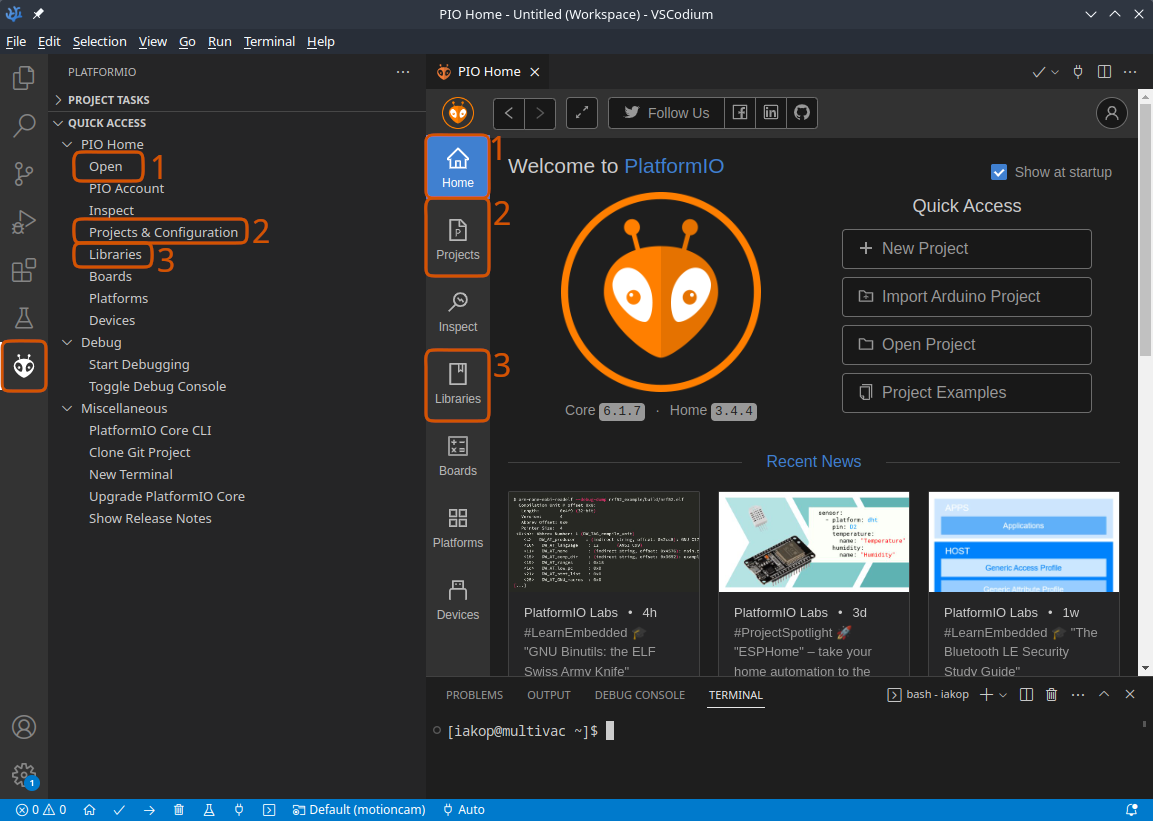
\includegraphics[width=\textwidth,keepaspectratio=true]{assets/pictures/pio-menu.png}
  			\caption{PlatformIO standard view, featuring \tthigh{Home}, \tthigh{Projects}, \tthigh{Libraries}, and Quick Access}
  			\label{fig:pio-menu}
		\end{figure}
	\end{column}
	\begin{column}{0.5\textwidth}
		\begin{textBox}
			\begin{itemize}
				\item The PlatformIO extension is opened by clicking the PlatformIO tab \includesvg[height=12pt, keepaspectratio=true]{assets/svg/pio-logo.svg}
				\item The most important menu items of the extension:
				\begin{enumerate}
					\item Open / Home
					\begin{itemize}
						\item Main page of PlatformIO, featuring quick access and tabs for most functions
					\end{itemize}
					\item Projects \& Configuration \\/ Projects
					\begin{itemize}
						\item Project management page, for creating and managing projects
					\end{itemize}
					\item Libraries
					\begin{itemize}
						\item For searching and adding Libraries to PlatformIO projects
					\end{itemize}
				\end{enumerate}
			\end{itemize}
		\end{textBox}
	\end{column}
\end{columns}
\end{frame}

\section{Setup of ESP32 project in PlatformIO}
\begin{frame}
	\sectiontitle{assets/svg/pio-logo.svg}{\insertsectionhead}
\end{frame}

\begin{frame}{Setup of ESP32 project in PlatformIO}
\begin{columns}
	\begin{column}{0.5\textwidth}
		\begin{textBox}
			\begin{itemize}
				\item Click the tab \tthigh{Projects} to enter the projects view
				\item To create a new project, click the button \tthigh{Create New Project}
			\end{itemize}
		\end{textBox}
	\end{column}
	\begin{column}{0.5\textwidth}
		\begin{figure}
  			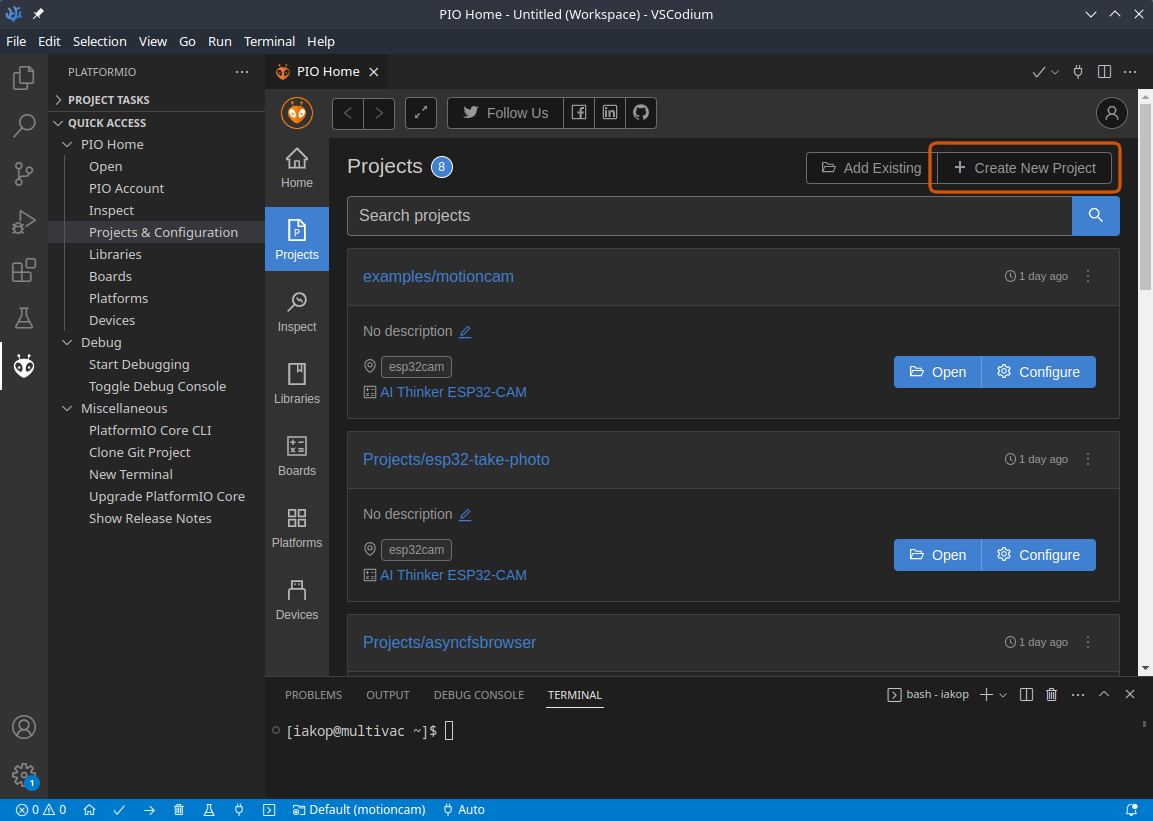
\includegraphics[width=\textwidth,keepaspectratio=true]{assets/pictures/pio-project.png}
  			\caption{\tthigh{Projects} tab in PlatformIO. For creating and managing projects within the GUI}
  			\label{fig:pio-project}
		\end{figure}
	\end{column}
\end{columns}
\end{frame}

\begin{frame}{Setup of ESP32 project in PlatformIO}
\begin{columns}
	\begin{column}{0.5\textwidth}
		\begin{figure}
  			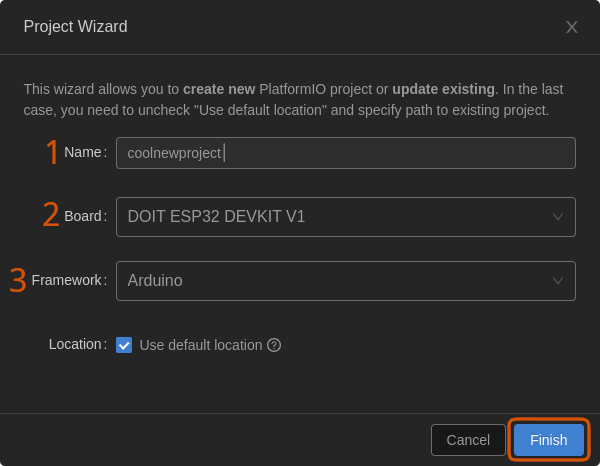
\includegraphics[height=0.7\textheight,keepaspectratio=true]{assets/pictures/pio-project-2.png}
  			\caption{The \tthigh{Project Wizard} dialog in PlatformIO, with settings for name, board and framework}
  			\label{fig:pio-project2}
		\end{figure}
	\end{column}
	\begin{column}{0.5\textwidth}
		\begin{textBox}
			\begin{itemize}
				\item A  \tthigh{Project Wizard} dialog will be opened
				\item It contains 3 fields, to be filled as follows:
				\begin{itemize}
					\item Name
					\begin{itemize}
						\item A fitting name for the project, e.g. "\tthigh{coolnewproject}"
					\end{itemize}
					\item Board
					\begin{itemize}
						\item \tthigh{DOIT ESP32 DEVKIT V1}
					\end{itemize}
					\item Framework
					\begin{itemize}
						\item \tthigh{Arduino}
					\end{itemize}
				\end{itemize}
				\item Finish by clicking \tthigh{Finish}
			\end{itemize}
		\end{textBox}
	\end{column}
\end{columns}
\end{frame}

\begin{frame}{Setup of ESP32 project in PlatformIO}
\begin{columns}
	\begin{column}{0.5\textwidth}
		\begin{textBox}
			\begin{itemize}
				\item PlatformIO will generate the project and set up the toolchain
				\begin{itemize}
					\item This requires an internet connection
				\end{itemize}
				\item When done, load \tthigh{platformio.ini}
				\begin{itemize}
					\item This file contains the project settings, and can be edited by hand
				\end{itemize}
				\item On the side of the window there are \tthigh{Project Tasks}:
				\begin{enumerate}
					\item Build
					\begin{itemize}
						\item Build an image for the device to be flashed
					\end{itemize}
					\item Upload
					\begin{itemize}
						\item Uploads the image through an automatically detected USB/UART connection
					\end{itemize}
					\item Monitor
					\begin{itemize}
						\item Monitors the UART connection to the hardware (Baud rate can be set in \tthigh{platformio.ini})
					\end{itemize}
					\item Build Filesystem Image
					\begin{itemize}
						\item Builds file system image for the hardware  (based on the contents of the \tthigh{data} folder of the project)
						\item \tthigh{data} folder needs to be created manually
						\item File system can be specified in \tthigh{platformio.ini}
					\end{itemize}
					\item Upload Filesystem Image
					\begin{itemize}
						\item Uploads the built image to the hardware
						\item \ttwarn{IMPORTANT}: Monitor can not be active during upload
					\end{itemize}
				\end{enumerate}
			\end{itemize}
		\end{textBox}
	\end{column}
	\begin{column}{0.5\textwidth}
		\begin{figure}
  			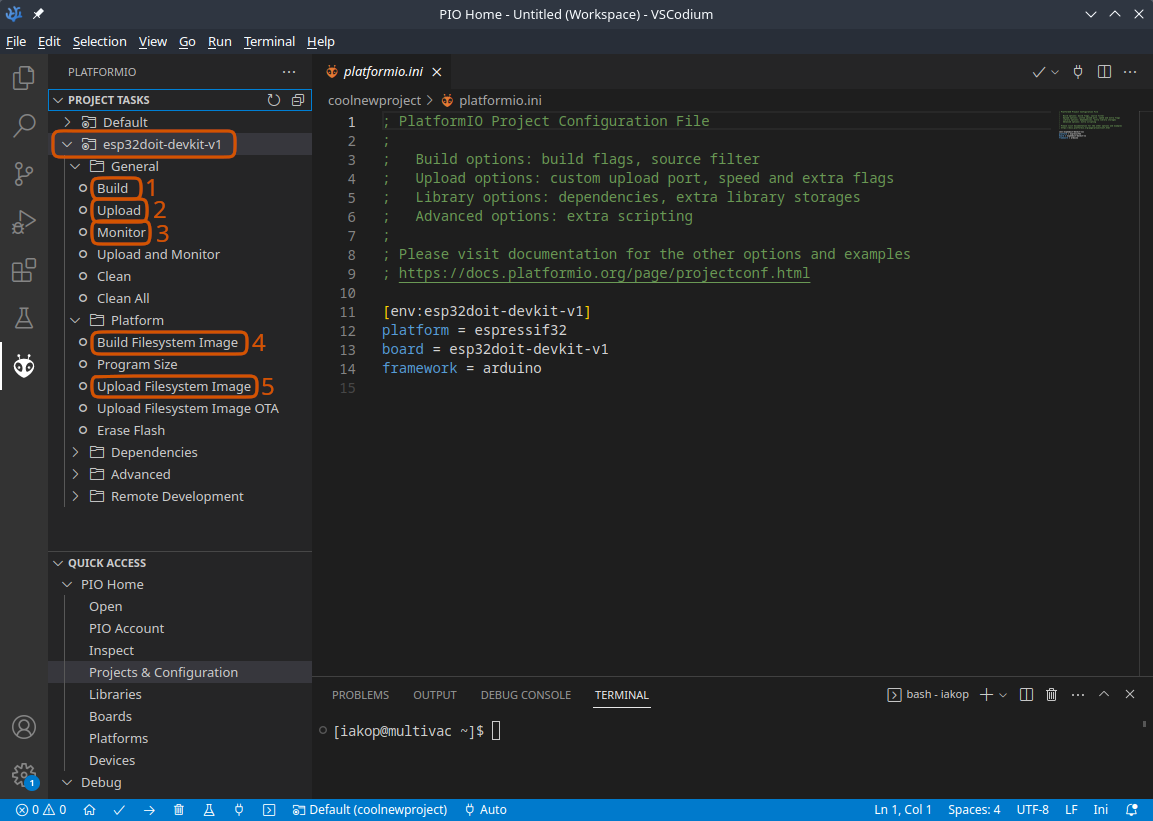
\includegraphics[width=\textwidth,keepaspectratio=true]{assets/pictures/pio-project-3.png}
  			\caption{Opened project in PlatformIO, shows \tthigh{platformio.ini} and the \tthigh{Project Tasks} for the project}
  			\label{fig:pio-project3}
		\end{figure}
	\end{column}
\end{columns}
\end{frame}

\subsection{Add libraries to an ESP32 project}
\begin{frame}{Add libraries to an ESP32 project}
\begin{columns}
	\begin{column}{0.5\textwidth}
		\begin{figure}
  			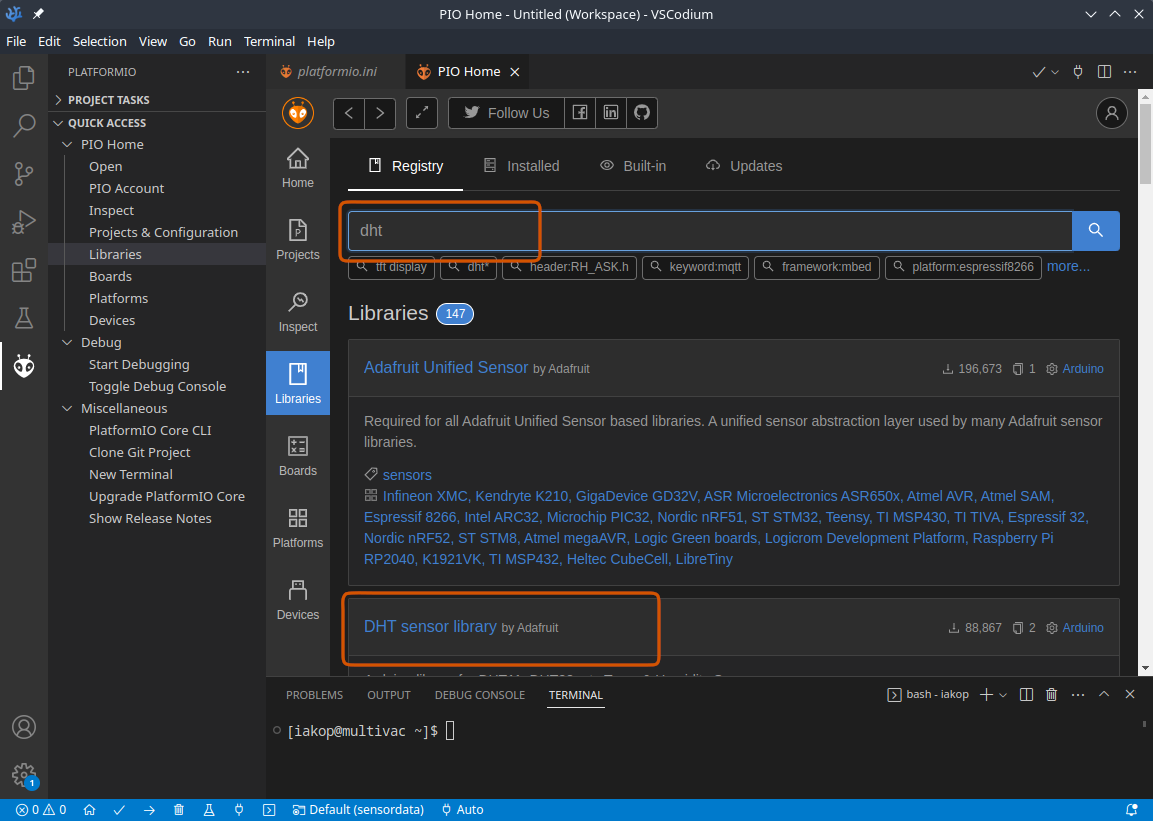
\includegraphics[width=\textwidth,keepaspectratio=true]{assets/pictures/pio-libraries.png}
  			\caption{The \tthigh{Libraries} tab in PlatformIO. For searching and adding libraries to projects}
  			\label{fig:pio-libraries}
		\end{figure}
	\end{column}
	\begin{column}{0.5\textwidth}
		\begin{textBox}
			\begin{itemize}
				\item To add external libraries to a project, use the \tthigh{Libraries} tab for finding contributed libraries
				\begin{itemize}
					\item Can be found under \tthigh{Registry}
					\item Installed libraries can be viewed underr \tthigh{Installed}
				\end{itemize}
				\item Click a relevant library
			\end{itemize}
		\end{textBox}
	\end{column}
\end{columns}
\end{frame}

\begin{frame}{Add libraries to an ESP32 project}
\begin{columns}
	\begin{column}{0.5\textwidth}
		\begin{textBox}
			\begin{itemize}
				\item The following can be found within the library:
				\begin{itemize}
					\item Examples
					\item Headers
					\item etc.
				\end{itemize}
				\item Click \tthigh{Add to Project} to add the library to a project
			\end{itemize}
		\end{textBox}
	\end{column}
	\begin{column}{0.5\textwidth}
		\begin{figure}
  			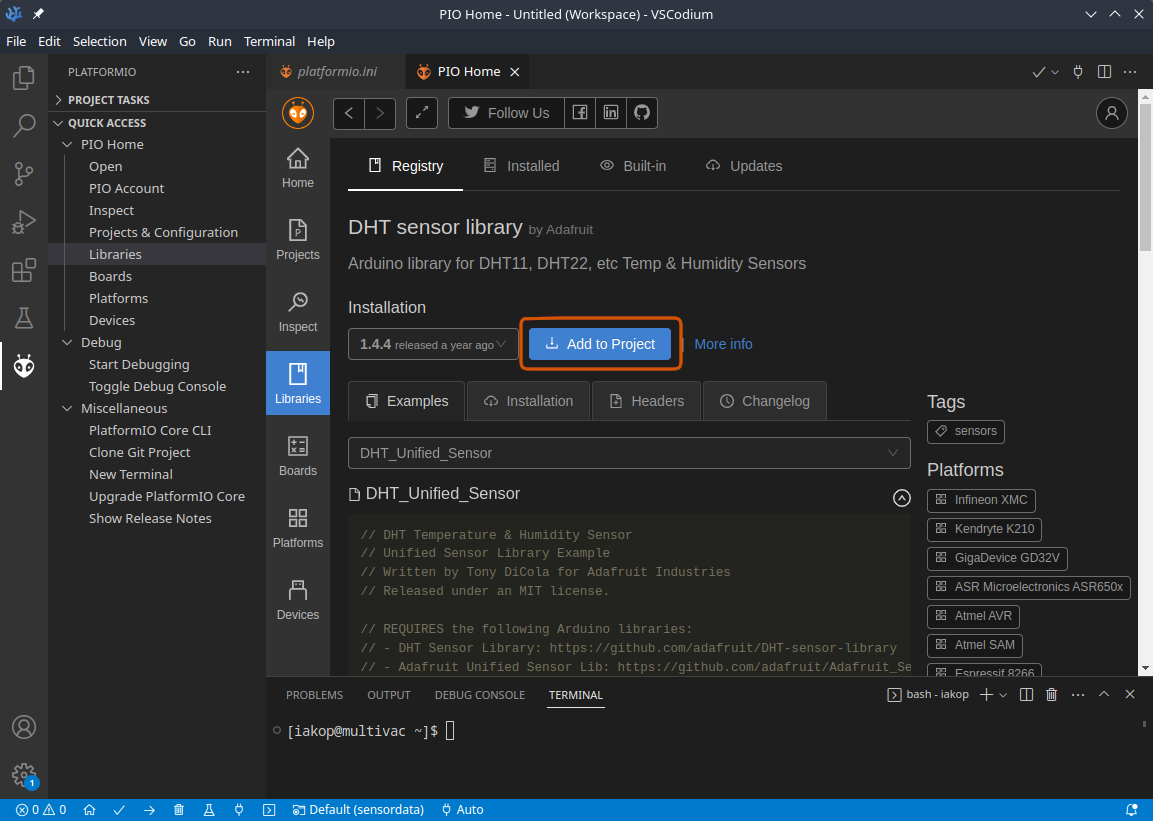
\includegraphics[width=\textwidth,keepaspectratio=true]{assets/pictures/pio-libraries-2.png}
  			\caption{\tthigh{DHT sensor library} in PlatformIO. Can be added to projects that support the Arduino framework}
  			\label{fig:pio-libraries-2}
		\end{figure}
	\end{column}
\end{columns}
\end{frame}

\begin{frame}{Add libraries to an ESP32 project}
\begin{columns}
	\begin{column}{0.5\textwidth}
		\begin{figure}
  			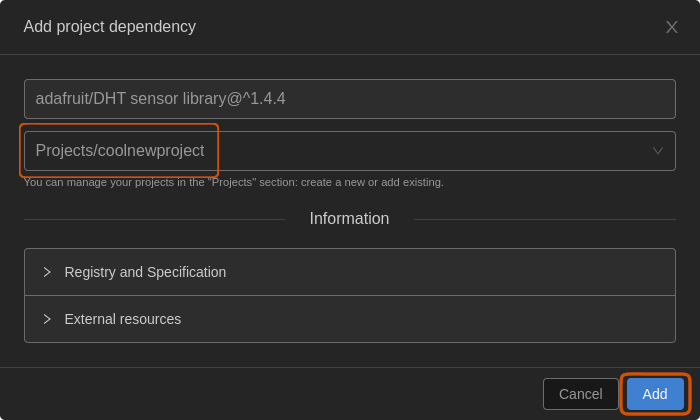
\includegraphics[width=\textwidth,keepaspectratio=true]{assets/pictures/pio-libraries-3.png}
  			\caption{The \tthigh{Add project dependency} dialog in PlatformIO. To pick which library to add the library to}
  			\label{fig:pio-libraries-3}
		\end{figure}
	\end{column}
	\begin{column}{0.5\textwidth}
		\begin{textBox}
			\begin{itemize}
				\item The \tthigh{Add project dependency} dialog will open
				\item Under \tthigh{Select a project}, pick the project to add the library to
				\item Click \tthigh{Add}
				\item PlatformIO will automatically add a \tthigh{lib\_deps} dependency within \tthigh{platformio.ini}, and set up the library
			\end{itemize}
		\end{textBox}
	\end{column}
\end{columns}
\end{frame}

\subsection{Opening external ESP32 Projekt in PlatformIO}
\begin{frame}{Opening external ESP32 Projekt in PlatformIO}
\begin{columns}
	\begin{column}{0.5\textwidth}
		\begin{figure}
  			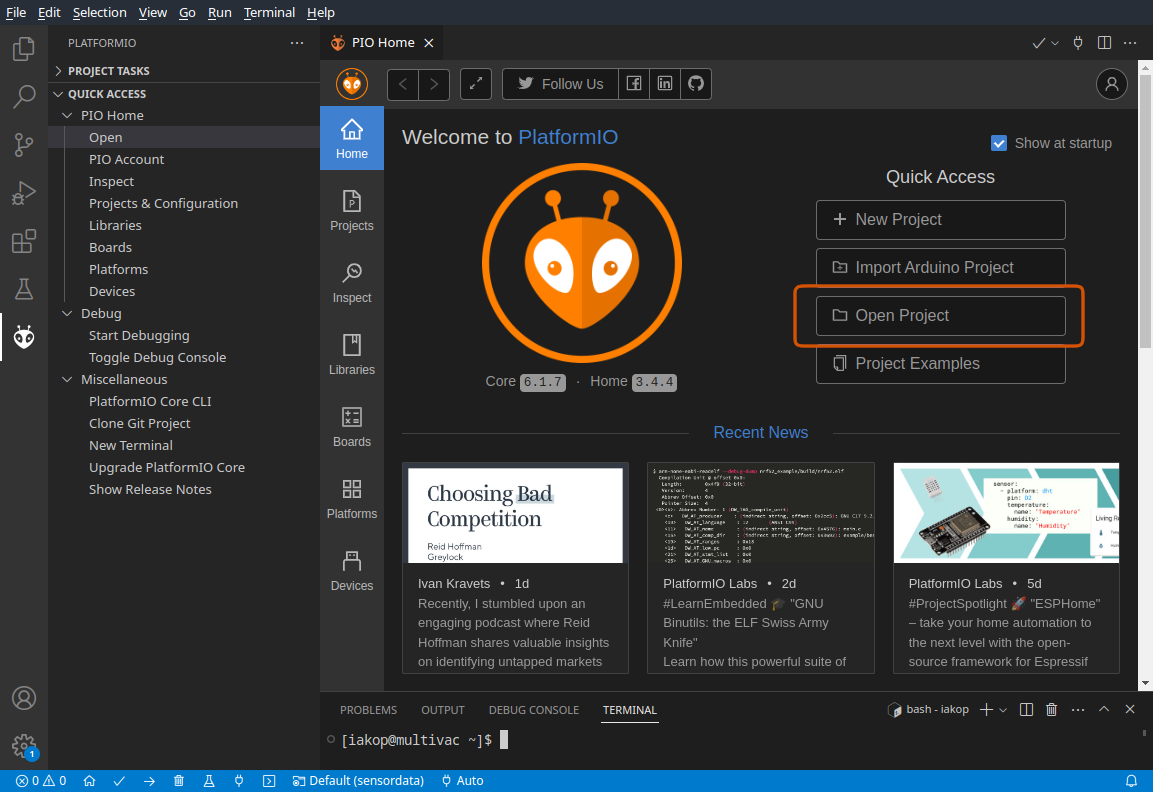
\includegraphics[width=\textwidth,keepaspectratio=true]{assets/pictures/pio-import.png}
  			\caption{\tthigh{Home} tab in PlatformIO, button to load project from disk is highlighted}
  			\label{fig:pio-project4}
		\end{figure}
	\end{column}
	\begin{column}{0.5\textwidth}
		\begin{textBox}
			\begin{itemize}
				\item The projects for this workshop use specific libraries and settings
				\item To get them quickly set up, the projects can be downloadet and imported from the Github repo
				\item Download the entire workshops materials here:
				\begin{itemize}
					\item \small\url{https://github.com/iakop/IoT-Crashcourse/archive/refs/heads/master.zip}
				\end{itemize}
				\item Extract them somewhere easy to locate
				\item Under the \tthigh{Home} tab, click \tthigh{Open Project}
			\end{itemize}
		\end{textBox}
	\end{column}
\end{columns}
\end{frame}

\begin{frame}{Opening external ESP32 Projekt in PlatformIO}
\begin{columns}
	\begin{column}{0.5\textwidth}
		\begin{textBox}
			\begin{itemize}
				\item In the \tthigh{Open PlatformIO Project} dialog, open the examples folder for the workshop
				\item If the \tthigh{Open} button, for example, shows \tthigh{Open "simpleServer"} the dialog is in the correct folder
				\item Click the \tthigh{Open} button
			\end{itemize}
		\end{textBox}
	\end{column}
	\begin{column}{0.5\textwidth}
		\begin{figure}
  			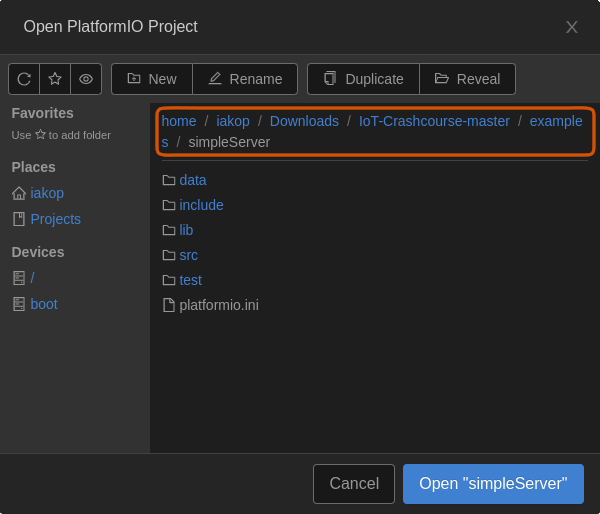
\includegraphics[height=0.7\textheight,keepaspectratio=true]{assets/pictures/pio-project-5.png}
  			\caption{\tthigh{Open PlatformIO Project} dialog in PlatformIO. To open a project the folder needs to be extracted and located on the disk, for example, in: \tthigh{Downloads/IoT-Crashcourse-master/examples/simpleServer}}
  			\label{fig:pio-project5}
		\end{figure}
	\end{column}
\end{columns}
\end{frame}

\begin{frame}{Opening external ESP32 Projekt in PlatformIO}
\begin{columns}
	\begin{column}{0.5\textwidth}
		\begin{figure}
  			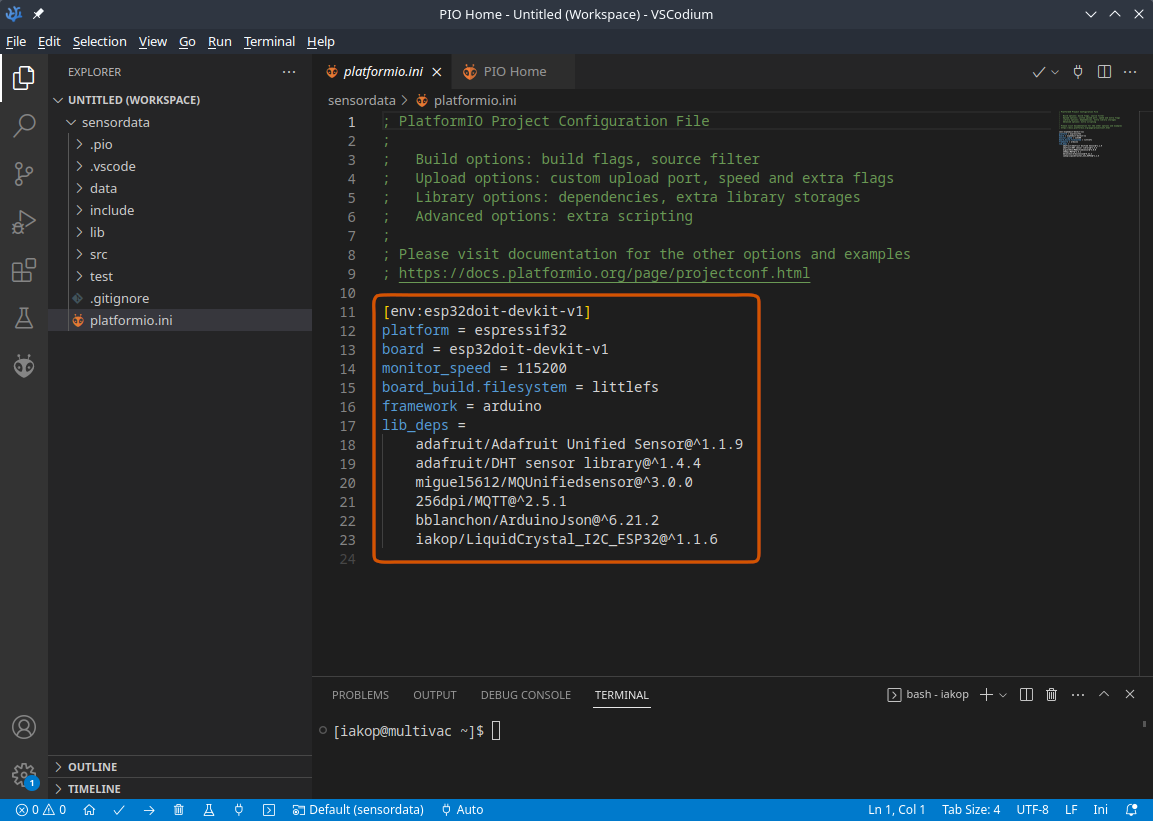
\includegraphics[width=\textwidth,keepaspectratio=true]{assets/pictures/pio-projects-6.png}
  			\caption{Example of a \tthigh{platformio.ini} for a project. Pay attention to \tthigh{monitor-speed}, \tthigh{filesystem} and \tthigh{lib\_deps} that are pre-defined}
  			\label{fig:pio-project6}
		\end{figure}
	\end{column}
	\begin{column}{0.5\textwidth}
		\begin{textBox}
			\begin{itemize}
				\item When the project is loaded, open the \tthigh{platformio.ini}
				\item Specifies libraries and components that the project depends on
				\item Tools and settings will be set up autimatically by PlatformIO
			\end{itemize}
		\end{textBox}
	\end{column}
\end{columns}
\end{frame}

\section{IoT basics}
\begin{frame}
	\sectiontitle{assets/svg/iot-star.svg}{\insertsectionhead}
\end{frame}

\begin{frame}{IoT basics}
\begin{columns}
	\begin{column}{0.6\textwidth}
		\begin{textBox}
			\begin{itemize}
				\item IoT (Internet of Things), is a common name for networked devices
				\item These devices typically consist of:
				\begin{itemize}
					\item A microprocessor or -computer
					\item Sensors
					\item Actuators
					\item Wired or wireless connectivity
				\end{itemize}
			\end{itemize}
		\end{textBox}
	\end{column}
	\begin{column}{0.4\textwidth}
		\centering
		\begin{figure}
			\captionsetup{format=tcbcaptionminmargin}
			\roundedGfx{0.9\textwidth}{assets/pictures/nedis-smartplug.jpg}
  			\caption{Nedis SmartLife torn down to show the insides. Contains a TYWE3S WiFi module and an HLW8012 power sensor
  			\captionline \textbf{Kilde:} \url{https://callaa.github.io/2021/01/26/liberating-nedis-smartplug.html}}
  			%\caption{Nedis SmartLife adskilt for at komme til indmaden. Indeholder bla. et TYWE3S WiFi modul og en HLW8012 effektsensor}
  			\label{fig:iot-device}
		\end{figure}
	\end{column}
\end{columns}
\end{frame}

\begin{frame}{IoT basics}
\begin{columns}
	\begin{column}{0.5\textwidth}
		\centering
		\captionsetup{format=tcbcaptionsmall}
		\begin{columns}
			\begin{column}{0.5\textwidth}
				\begin{figure}[height=0.2\textheight]
  					\includesvg[height=0.2\textheight]{assets/svg/iot-star.svg}
  					\caption{Star-topology, where every device communicates through a central gateway to the rest of the internet}
  					\label{fig:iot-star}
				\end{figure}
			\end{column}
			\begin{column}{0.5\textwidth}
				\begin{figure}[height=0.2\textheight]
  					\includesvg[height=0.2\textheight]{assets/svg/iot-tree.svg}
  					\caption{Tree-topology, Where the devices are connected in branches, where they heirarchically relay information to the gateway}
  					\label{fig:iot-tree}
				\end{figure}
			\end{column}
		\end{columns}
		\begin{columns}
			\begin{column}{0.5\textwidth}
				\begin{figure}[height=0.2\textheight]
  					\includesvg[height=0.2\textheight]{assets/svg/iot-mesh.svg}
  					\caption{Mesh-topology, where devices communicate internally, relaying information through eachother to the gateway}
  					\label{fig:iot-mesh}
				\end{figure}
			\end{column}
		\end{columns}
	\end{column}
	\begin{column}{0.5\textwidth}
		\begin{textBox}
			\begin{itemize}
				\item Communication between devices can be done in several ways
				\item Some typical IoT toplogies:
				\begin{itemize}
					\item Star
					\item Tree
					\item Mesh
				\end{itemize}
			\end{itemize}
		\end{textBox}
	\end{column}
\end{columns}
\end{frame}

\begin{frame}{IoT basics}
\begin{columns}
	\begin{column}{0.6\textwidth}
		\begin{textBox}
			\begin{itemize}
				\item There are also several protocols for devices to communicate
				\item In this workshop we focus on:
				\begin{itemize}
					\item HTTP
						\begin{itemize}
							\item The ubiquitous Hypertext Transfer Protocol, for transferring web content, e.g. between servers and browsers
						\end{itemize}
					\item WebSocket
						\begin{itemize}
							\item A full duplex (two-way communication) protocol for quick, simultaneous communication between client and server - low overhead
						\end{itemize}
					\item MQTT
						\begin{itemize}
							\item (Originally acronym for MQ (Message Queue) Telemetry Transport) Publish-subscribe based protocol between devices and a central broker - low overhead
						\end{itemize}
				\end{itemize}
			\end{itemize}
		\end{textBox}
	\end{column}
	\begin{column}{0.4\textwidth}
		\centering
		\captionsetup{format=tcbcaptionsmall}
		\begin{columns}
			\begin{column}{0.45\textwidth}
				\begin{figure}[height=0.2\textheight]
  					\includesvg[height=0.2\textheight]{assets/svg/http-logo.svg}
  					\caption{HTTP logo
  					\captionline \textbf{Kilde:} \url{https://en.wikipedia.org/wiki/File:HTTP_logo.svg}
  					\captionline \textbf{Licens:} Public Domain}
  					\label{fig:http-logo}
				\end{figure}
			\end{column}
			\begin{column}{0.45\textwidth}
				\begin{figure}[height=0.2\textheight]
  					\includesvg[height=0.2\textheight]{assets/svg/websocket-logo.svg}
  					\caption{WebSocket logo
  					\captionline \textbf{Kilde:} \url{https://logodix.com/logos/1825947}
  					\captionline \textbf{Licens:} Non-Commercial}
  					\label{fig:websocket-logo}
				\end{figure}
			\end{column}
		\end{columns}
		\begin{columns}
			\begin{column}{0.45\textwidth}
				\begin{figure}[height=0.2\textheight]
  					\includesvg[height=0.2\textheight]{assets/svg/mqtt-logo.svg}
  					\caption{MQTT logo
  					\captionline \textbf{Kilde:} \url{https://en.wikipedia.org/wiki/File:Mqtt-hor.svg}
  					\captionline \textbf{Licens:} Public Domain}
  					\label{fig:mqtt-logo}
				\end{figure}
			\end{column}
		\end{columns}
	\end{column}
\end{columns}
\end{frame}

\section{Build a simple ESP32 webserver}
\begin{frame}
	\sectiontitle{assets/pictures/simpleserver.png}{\insertsectionhead}
\end{frame}

\subsection{Eksempel: Simple Server}
\begin{frame}{Simple Server}
\begin{columns}
	\begin{column}{0.6\textwidth}
		\begin{textBox}
		\begin{itemize}
			\item For this example we need a breadboard setup
			\begin{itemize}
				\item An ESP32 board
				\item An LED
				\item A 220{\textsf{$\Omega$}} resistor
			\end{itemize}
			\item HTML and the Arduino program will be presented and explained on the board
			%\captionbreak
			\item Source code can be found on:
			\begin{itemize}
				\item \tiny\url{https://github.com/iakop/IoT-Crashcourse/tree/master/examples/simpleServer}
			\end{itemize}
		\end{itemize}
		\end{textBox}
	\end{column}
	\begin{column}{0.4\textwidth}
		\centering
		\begin{figure}
  			\includesvg[height=0.6\textheight]{assets/setups/esp32-led.svg}
  			\caption{Breadboard setup with ESP32 and LED}
  			\label{fig:esp32-led}
		\end{figure}
	\end{column}
\end{columns}
\end{frame}

\section{WebSockets on ESP32}
\begin{frame}
	\sectiontitle{assets/pictures/websocketserver.png}{\insertsectionhead}
\end{frame}

\subsection{Eksempel: WebSocket Server}
\begin{frame}{WebSocket Server}
\begin{columns}
	\begin{column}{0.6\textwidth}
		\begin{textBox}
		\begin{itemize}
			\item This example adds a sensor to the setup
			\begin{itemize}
				\item An ESP32 board
				\item An LED
				\item A 220{\textsf{$\Omega$}} resistor
				\item A DHT11 temperature/humidity sensor module
			\end{itemize}
			\item We'll add Javascript and a WebSocket connection, which we'll also cover on the board
			\item Source code can be found on:
			\begin{itemize}
				\item \tiny\url{https://github.com/iakop/IoT-Crashcourse/tree/master/examples/websocketServer}
			\end{itemize}
		\end{itemize}
		\end{textBox}
	\end{column}
	\begin{column}{0.4\textwidth}
		\centering
		\begin{figure}
  			\includesvg[height=0.6\textheight]{assets/setups/esp32-led-dht11.svg}
  			\caption{Breadboard setup with ESP32, LED and DHT11 sensor}
  			\label{fig:esp32-led-dht11}
		\end{figure}
	\end{column}
\end{columns}
\end{frame}

\section{MQTT on ESP32}
\begin{frame}
	\sectiontitle{assets/pictures/mqttclient.png}{\insertsectionhead}
\end{frame}

\subsection{Eksempel: MQTT Client}
\begin{frame}{MQTT Client}
\begin{columns}
	\begin{column}{0.6\textwidth}
		\begin{textBox}
		\begin{itemize}
			\item Same setup
			\begin{itemize}
				\item An ESP32 board
				\item An LED
				\item A 220{\textsf{$\Omega$}} resistor
				\item A DHT11 temperature/humidity sensor module
			\end{itemize}
			\item All server code is exchanged for client code, connecting through SSL to an MQTT broker
			\item Source code can be found on:
			\begin{itemize}
				\item \tiny\url{https://github.com/iakop/IoT-Crashcourse/tree/master/examples/mqttClient}
			\end{itemize}
		\end{itemize}
		\end{textBox}
	\end{column}
	\begin{column}{0.4\textwidth}
		\centering
		\begin{figure}
  			\includesvg[height=0.6\textheight]{assets/setups/esp32-led-dht11.svg}
  			\caption{Breadboard setup with ESP32, LED and DHT11 sensor}
  			\label{fig:esp32-led-dht11-2}
		\end{figure}
	\end{column}
\end{columns}
\end{frame}

\begin{frame}{MQTT Client}
\begin{columns}
\begin{column}{0.6\textwidth}
		\centering
		\begin{figure}
  			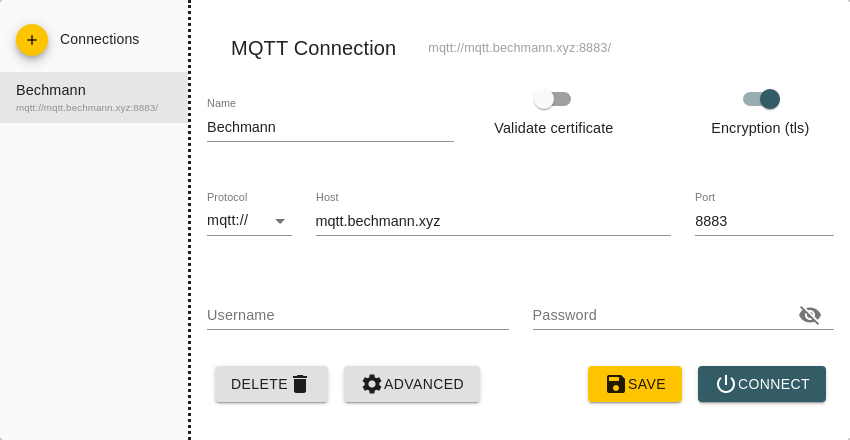
\includegraphics[width=\textwidth]{assets/pictures/mqtt-explorer.png}
  			\caption{MQTT Explorer Connection dialog window, with the settings for connecting to \tthigh{mqtt.bechmann.xyz}}
  			\label{fig:mqtt-explorer}
		\end{figure}
	\end{column}
	\begin{column}{0.4\textwidth}
		\begin{textBox}
		\begin{itemize}
			\item MQTT Explorer can be used to check and explore topics on a broker:
			\begin{itemize}
				\item \small\url{http://mqtt-explorer.com/}
			\end{itemize}
			\item Settings for \ttwarn{public} server for this workshop:
			\begin{itemize}
				\item Name: \tthigh{Bechmann} (optional)	
				\item Validate certificate:	 \tthigh{off} 
				\begin{itemize}
					\item \ttlow{Bug in MQTT Explorers cert storage prevents validating Let's Encrypt RootCA}
				\end{itemize}
				\item Encryption (tls):	 \tthigh{on} 
				\item Protocol: \tthigh{mqtt://}
				\item Host: \tthigh{mqtt.bechmann.xyz}
				\item Port: \tthigh{8883}
				\item Username: \ttlow{blank}
				\item Password: \ttlow{blank}
			\end{itemize}
		\end{itemize}
		\end{textBox}
	\end{column}
\end{columns}
\end{frame}

\end{document}